% Created 2020-11-19 Thu 21:24
% Intended LaTeX compiler: pdflatex
\documentclass[11pt]{article}
\usepackage[utf8]{inputenc}
\usepackage[T1]{fontenc}
\usepackage{graphicx}
\usepackage{grffile}
\usepackage{longtable}
\usepackage{wrapfig}
\usepackage{rotating}
\usepackage[normalem]{ulem}
\usepackage{amsmath}
\usepackage{textcomp}
\usepackage{amssymb}
\usepackage{capt-of}
\usepackage{hyperref}
\usepackage[russian]{babel}
\usepackage{amsmath}
\usepackage{esint}
\usepackage{mathtools}
\usepackage{amsthm}
\usepackage[top=0.8in, bottom=0.75in, left=0.625in, right=0.625in]{geometry}
\usepackage{dot2texi}
\usepackage{tikz}
\usetikzlibrary{shapes, arrows, positioning}
\def\zall{\setcounter{lem}{0}\setcounter{cnsqnc}{0}\setcounter{th}{0}\setcounter{Cmt}{0}\setcounter{equation}{0}\setcounter{stnmt}{0}}
\newcounter{lem}\setcounter{lem}{0}
\def\lm{\par\smallskip\refstepcounter{lem}\textbf{\arabic{lem}}}
\newtheorem*{Lemma}{Лемма \lm}
\newcounter{th}\setcounter{th}{0}
\def\th{\par\smallskip\refstepcounter{th}\textbf{\arabic{th}}}
\newtheorem*{Theorem}{Теорема \th}
\newcounter{cnsqnc}\setcounter{cnsqnc}{0}
\def\cnsqnc{\par\smallskip\refstepcounter{cnsqnc}\textbf{\arabic{cnsqnc}}}
\newtheorem*{Consequence}{Следствие \cnsqnc}
\newcounter{Cmt}\setcounter{Cmt}{0}
\def\cmt{\par\smallskip\refstepcounter{Cmt}\textbf{\arabic{Cmt}}}
\newtheorem*{Note}{Замечание \cmt}
\newcounter{stnmt}\setcounter{stnmt}{0}
\def\st{\par\smallskip\refstepcounter{stnmt}\textbf{\arabic{stnmt}}}
\newtheorem*{Statement}{Утверждение \st}
\author{Sergey Makarov}
\date{\today}
\title{}
\hypersetup{
 pdfauthor={Sergey Makarov},
 pdftitle={},
 pdfkeywords={},
 pdfsubject={},
 pdfcreator={Emacs 27.1 (Org mode 9.4)}, 
 pdflang={Russian}}
\begin{document}

\tableofcontents


\section{Домашняя работа 1}
\label{sec:orgf762115}
\subsection{Упражнение 1.2}
\label{sec:org6c6dbe4}
Используя приведённые ниже предикаты:
\begin{enumerate}
\item \(C(x)\) -- "\(x\) -- квадрат";
\item \(S(x)\) -- "\(x\) -- шар";
\item \(B(x)\) -- "\(x\) -- чёрный предмет";
\item \(W(x)\) -- "\(x\) -- белый предмет";
\item \(U(x, y)\) -- "предмет \(x\) лежит ниже предмета \(y\)";
\end{enumerate}
Записать формулы для утверждений:
\begin{enumerate}
\item "Хотя бы один квадрат, лежащий ниже всех чёрных квадратов, не является шаром";
\item "Нет такого белого квадрата, который лежит под каким-то чёрным шаром";
\item "Каков бы ни был чёрный предмет, либо он является шаром, лежащим выше всех белых квадратов, либо он является квадратом, лежащим ниже какого-нибудь шара";
\item "Никакой чёрный квадрат и никакой белый шар не лежат друг над другом";
\item "Если все шары чёрные, то белых квадратов нет";
\item "Всякая фигура, не являющаяся белым квадратом, лежащим хотя бы над одним шаром, имеет чёрный цвет и лежит над всеми белыми фигурами";
\end{enumerate}
\subsubsection{Решение}
\label{sec:org3629baf}
\begin{enumerate}
\item \(\exists x (C(x) \land (\forall y (C(y) \land B(y) \land U(x, y))) \to \lnot S(x))\).
\item \(\lnot \exists x (W(x) \land C(x) \land \exists y (S(y) \land B(y) \land U(x, y)))\).
\item \(\forall x (B(x) \to S(x) \land (\forall y (W(y) \land C(y) \to U(y, x))) \lor C(x) \land \exists y (S(y) \land U(x, y)))\).
\item \(\forall x \forall y (B(x) \land C(x) \land S(y) \land W(y) \to \neg U(x, y) \land \neg U(y, x))\).
\item \(\forall x (S(x) \to B(x)) \to \lnot \exists x (W(x) \land C(x))\).
\item \(\forall x (\lnot (W(x) \land C(x) \land \exists y (S(y) \land U(y, x))) \to B(x) \land \forall y (W(y) \to U(y, x)))\).
\end{enumerate}

\subsection{Упражнение 2}
\label{sec:orgca7b6be}
Записать формулу в логике правил арифметики со свободной переменной \(x\), истинную в интерпретации на натуральных числах тогда и только тогда, когда \(x\) -- простое число.
\subsubsection{Решение}
\label{sec:orgad4dbf9}
По определению, число является простым тогда и только тогда, когда оно имеет ровно два делителя: единицу и себя самого. Число 1 при этом простым не является. Используя предикаты из условия, это можно записать так:
\begin{equation*}
Pr(x) = \lnot \phi_1(x) \land \forall y (\exists z P(y, z, x) \to \phi_1(y) \lor Eq(y, x))
\end{equation*}
Здесь
\begin{gather*}
\phi_0(t) = S(t, t, t), \\
\phi_1(t) = P(t, t, t) \land \lnot \phi_0(t), \\
Eq(x, y) = \forall t (S(x, t, y) \lor S(y, t, x) \to \phi_0(t))
\end{gather*}
\pagebreak
\section{Домашняя работа 2}
\label{sec:org6436c23}
\subsection{Упражнение 2.1}
\label{sec:org3a2951f}
Установить, являются ли приведённые формулы:
\begin{enumerate}
\item выполнимыми
\item общезначимыми
\item невыполнимыми:
\begin{itemize}
\item \(\exists x P(x) \land \exists x \lnot P(x)\)
\item \(\exists x P(x) \lor \exists x \lnot P(x)\)
\item \(\exists x\forall y(P(x) \land \lnot P(y))\)
\item \(P(x) \to \forall x P(x)\)
\item \(\forall x P(x) \to P(x)\)
\item \(\forall y\exists x R(x, y) \to \exists x\forall y R(x, y)\)
\item \((\forall x P(x) \to \forall x Q(x)) \to \forall x (P(x) \to Q(x))\)
\end{itemize}
\end{enumerate}
\subsubsection{Решение}
\label{sec:org8e5005d}
    \begin{equation*}
\varphi = \exists x P(x) \land \exists x \lnot P(x)
    \end{equation*}
Эта формула является выполнимой. Рассмотрим интерпретацию \(I_1\), в которой:
\begin{align*}
D = \{d_1, d_2\}, P(d_1) = \textbf{true}, P(d_2) = \textbf{false}.
\end{align*}
В этой интерпретации формула верна.

Рассмотрим теперь интерпретацию $I_2$, в которой:
\begin{align*}
D = \{d_1\}, P(d_1) = \textbf{true}
\end{align*}
В этой интерпретации формула неверна.

\begin{equation*}
\varphi = \exists x P(x) \lor \exists x \lnot P(x)
\end{equation*}

Эта формула является общезначимой. Пусть эта формула не выполняется в интерпретации \(I\). Тогда:
\begin{align*}
I \not \models \exists x P(x) \lor \exists x \lnot P(x) \\
I \models \forall x P(x) \land \forall x \lnot P(x)
\end{align*}
Получили противоречие. Значит формула $\lnot\varphi$ невыполнима и формула $\phi$ общезначима.

\begin{equation*}
\varphi = \exists x \forall y (P(x) \land \lnot P(y))
\end{equation*}

Эта формула невыполнима. В самом деле, рассмотрим произвольную непустую интерпретацию \(I\), в которой эта формула выполняется. Тогда \(\exists d \in D\), такое что для него выполнены одновременно \(P(x)\) и \(\lnot P(x)\), что невозможно.

\begin{equation*}
\varphi = P(x) \to \forall x P(x)
\end{equation*}

Эта формула выполнима. Рассмотрим интерпретацию \(I_1\):
\begin{align*}
D = \{d_1\}, P(d_1) = \textbf{true}
\end{align*}
В этой интерпретации формула выполнена. В интерпретации $I_2$:
\begin{align*}
D = \{d_1, d_2\}, P(d_1) = \textbf{true}, P(d_2) = \textbf{false}
\end{align*}
формула не выполнена.

\begin{equation*}
\varphi = \forall x P(x) \to P(x)
\end{equation*}

Эта формула является общезначимой. В самом деле, пусть интерпретация \(I\) опровергает эту формулу. Тогда:
\begin{align*}
I \not\models \forall x P(x) \to P(x) \\
I \models \forall x P(x), \lnot P(x)
\end{align*}
Получили противоречие. Значит, формула $\varphi$ является общезначимой.

\begin{equation*}
\forall y\exists x R(x, y) \to \exists x \forall y R(x, y)
\end{equation*}

Эта формула является выполнимой. Рассмотрим интерпретацию \(I_1\):
\begin{align*}
D = \{d\}, R(d, d) = \textbf{true}
\end{align*}
В этой интерпретации формула выполнена. В интерпретации $I_2$:
\begin{align*}
D = \{d_1, d_2\}, R(d_1, d_1) = R(d_2, d_2) = \textbf{true}, R(d_1, d_2) = R(d_2, d_1) = \textbf{false}
формула не выполнена.
\end{align*}

\begin{equation*}
(\forall x P(x) \to \forall x Q(x)) \to \forall x(P(x) \to Q(x))
\end{equation*}

Эта формула общезначима. В самом деле, пусть интерпретация \(I\) опровергает эту формулу. Тогда:
\begin{align*}
I \not\models (\forall x P(x) \to \forall x Q(x)) \to \forall x(P(x) \to Q(x)) \\
I \models (\forall x P(x) \to \forall x Q(x)) &\, I \not\models (\forall x (P(x) \to Q(x))) \\
I \models \exists x \lnot (P(x) \to Q(x)) \\
I \models \exists x P(x) \land \lnot Q(x) [d] \\
I \models P(d) \\
I \models \lnot Q(d) \\
I \models P(d) \to Q(d) \\
I \models Q(d)
\end{align*}
Получили противоречие. Значит, формула $\varphi$ общезначима.
\subsection{Упражнение 2.2 (1-5, 7, 9)}
\label{sec:orgd22f128}
Применяя табличный вывод, обосновать общезначимость формул:
\begin{enumerate}
\item \(\exists x P(x) \to \lnot \forall x \lnot P(x)\)
\item \(\exists x \forall y R(x, y) \to \forall y \exists x R(x, y)\)
\item \(\forall x (P(x) \to \exists y R(x, f(y))) \to (\exists x \lnot P(x) \lor \forall x \exists z R(x, z))\)
\item \(\forall x \exists y \forall z (P(x, y) \to P(y, z))\)
\item \(\exists x \forall y \exists z (P(x, y) \to P(y, z))\)
\item \((\forall x P(x) \land \forall x R(x)) \to \forall x (P(x) \land R(x))\)
\item \((\exists x P(x) \lor \exists x R(x)) \to \exists x (P(x) \lor R(x))\)
\end{enumerate}
\subsubsection{Решение}
\label{sec:org3e5a5ee}
\begin{enumerate}
\item \(\exists x P(x) \to \lnot \forall x \lnot P(x)\)
\end{enumerate}
Пусть интерпретация \(I\) опровергает эту формулу. Тогда:
\begin{gather*}
I \not\models \exists x P(x) \to \lnot\forall x \lnot P(x) \\
I \models \exists x P(x)[d] \\
I \not\models \lnot\forall x \lnot P(x) \\
I \models \forall x \lnot P(x) \\
I \models P(d) \\
I \models \lnot P(d)
\end{gather*}
Получили противоречие. Значит, исходная формула общезначима.

\begin{enumerate}
\item \(\exists x \forall y R(x, y) \to \forall y \exists x R(x, y)\)
\end{enumerate}
Пусть интерпретация \(I\) опровергает эту формулу. Тогда:
\begin{gather*}
I \not\models \exists x\forall y R(x, y) \to \forall y \exists x R(x, y) \\
I \models \exists x \forall y R(x, y)[d] \\
I \not\models \forall y \exists x R(x, y) \\
I \models \forall y R(d, y) \\
I \models \exists y \forall x \lnot R(x, y) \\
I \models \exists y \lnot R(d, y)[d_2] \\
I \models \lnot R(d, d_2) \\
I \models R(d, d_2)
\end{gather*}
Получили противоречие. Значит, исходная формула общезначима.

\begin{enumerate}
\item \(\forall x(P(x) \to \exists y R(x, f(y))) \to (\exists x \lnot P(x) \lor \forall x \exists z R(x, z))\)
\end{enumerate}
Пусть интерпретация \(I\) опровергает эту формулу. Тогда:
\begin{gather*}
\Gamma = \emptyset, \Delta = \{\forall x (P(x) \to \exists y R(x, f(y))) \to \exists x \lnot P(x) \lor \forall x \exists z R(x, z)\} \Rightarrow_{R_\to} \\
\Gamma = \{\forall x(P(x) \to \exists y R(x, f(y)))\}, \Delta = \{\exists x \lnot P(x)\lor\forall x\exists z R(x, z)\} \Rightarrow_{R_\lor} \\
\Gamma = \{\forall x(P(x) \to \exists y R(x, f(y)))\}, \Delta = \{\exists x \lnot P(x), \forall x \exists z R(x, z)\} \Rightarrow_{R_\forall} \\
\Gamma = \{\forall x (P(x) \to \exists y R(x, f(y)))\}, \Delta = \{\exists x \lnot P(x), \exists z R(a, z)\} \Rightarrow_{L_\forall} \\
\Gamma = \{\forall x (P(x) \to \exists y R(x, f(y))), (P(x) \to \exists y R(x, f(y)))[x / t]\}, \Delta = \{\exists x\lnot P(x), \exists z R(a, z)\} \Rightarrow_{R_\exists} \\
\Gamma = \{\forall x (P(x) \to \exists y R(x, f(y))), (P(x) \to \exists y R(x, f(y)))[x / t]\}, \Delta = \{\exists x \lnot P(x), (\lnot P(x))[x / t], \exists z R(a, z)\} \Rightarrow_{R_\exists} \\
\Gamma = \{\forall x (P(x) \to \exists y R(x, f(y))), (P(x) \to \exists y R(x, f(y)))[x / t]\}, \\
\Delta = \{\exists x \lnot P(x), (\lnot P(x))[x / t], \exists z R(a, z), R(a, z)[z / t]\} \Rightarrow_{L_\to} \\
\Gamma = \{\forall x (P(x) \to \exists y R(x, f(y))), \exists y R(x, f(y))[x / t]\}, \Delta = \{\exists x \lnot P(x), (\lnot P(x))[x / t], \exists z R(a, z), R(a, z)[z / t]\} \Rightarrow_{L_\exists} \\
\Gamma = \{\forall x (P(x) \to \exists y R(x, f(y))), R(x, f(c))[x / t]\}, \Delta = \{\exists x \lnot P(x), (\lnot P(x))[x / t], \exists z R(a, z), R(a, z)[z / t]\} \Rightarrow_{x \to a, z \to f(c)} \\
\Gamma = \{\forall x (P(x) \to \exists y R(x, f(y))), R(x, f(c))[x / t], R(a, f(c))\}, \\
\Delta = \{\exists x \lnot P(x), (\lnot P(x))[x / t], \exists z R(a, z), R(a, z)[z / t], R(a, f(c))\} \, (?!) \\
\Gamma = \{\forall x (P(x) \to \exists y R(x, f(y)))\}, \Delta = \{\exists x \lnot P(x), (\lnot P(x))[x / t], \exists z R(a, z), R(a, z)[z / t], P(x)[x / t]\} \, (?!)
\end{gather*}
Получили противоречие. Значит, формула общезначима.

\begin{enumerate}
\item \(\forall x \exists y \forall z (P(x, y) \to P(y, z))\).
\end{enumerate}

Пусть интерпретация \(I\) опровергает эту формулу. Тогда:
\begin{gather*}
T = <\emptyset | \forall x \exists y \forall z (P(x, y) \to P(y, z))> \Rightarrow_{\forall_R} \\
T = <\emptyset | \exists y \forall z (P(a, y) \to P(y, z))> \Rightarrow_{\exists_R} \\
T = <\emptyset | (\forall z (P(a, y) \to P(y, z)))[y/t], \exists y \forall z (P(a, y) \to P(y, z))> \Rightarrow_{\forall_R} \\
T = <\emptyset | (P(a, y) \to P(y, b))[y/t], \exists y\forall z(P(a, y) \to P(y, z))> \Rightarrow_{\to_R} \\
T = <P(a, y)[y/t] | P(y, b)[y/t], \exists y \forall z (P(a, y) \to P(y, z))> \Rightarrow_{y \to a} \\
T = <P(a, a), P(a, y)[y/t] | P(a, b), P(y, b)[y/t], \exists y \forall z (P(a, y) \to P(y, z))> \Rightarrow_{y \to b} \\
T = <P(a, a), P(a, b), P(a, y)[y/t] | P(a, b), P(b, b), P(y, b)[y/t], \exists y \forall z (P(a, y) \to P(y, z))
\end{gather*}
Получили закрытую таблицу $\Rightarrow$ формула общезначима.

\begin{enumerate}
\item \(\exists x \forall y \exists z (P(x, y) \to P(y, z))\)
\end{enumerate}

Пусть интерпретация \(I\) опровергает эту формулу. Тогда:
\begin{gather*}
T = <\emptyset | \exists x \forall y \exists z (P(x, y) \to P(y, z))> \Rightarrow_{\exists_R} \\
T = <\emptyset | (\forall y \exists z (P(x, y) \to P(y, z)))[x/t_1], \exists x \forall y \exists z (P(x, y) \to P(y, z))> \Rightarrow_{\forall_R} \\
T = <\emptyset | (\exists z (P(x, a) \to P(a, z)))[x/t_1], \exists x \forall y \exists z (P(x, y) \to P(y, z))> \Rightarrow_{\exists_R} \\
T = <\emptyset | (P(x, a) \to P(a, z))[x/t_1, z/t_2], (\exists z (P(x, a) \to P(a, z)))[x/t_1], \exists x \forall y \exists z (P(x, a) \to P(a, z))> \Rightarrow_{\to_R} \\
T = <P(x, a)[x/t_1, z/t_2] | P(a, z)[x/t_1, z/t_2], (\exists z (P(x, a) \to P(a, z)))[x/t_1], \exists x \forall y \exists z (P(x, a) \to P(a, z))> \Rightarrow_{x \to a, z \to a} \\
T = <P(a, a), P(x, a)[x/t_1, z/t_2] | P(a, a), P(a, z)[x/t_1, z/t_2], (\exists z (P(x, a) \to P(a, z)))[x/t_1], \exists x \forall y \exists z (P(x, a) \to P(a, z))>
\end{gather*}
Получили закрытую таблицу $\Rightarrow$ формула общезначима.

\begin{enumerate}
\item \((\forall x P(x) \land \forall x R(x)) \to \forall x(P(x) \land R(x))\)
\end{enumerate}

Пусть интерпретация \(I\) опровергает эту формулу. Тогда:
\begin{gather*}
T = <\emptyset | (\forall x P(x) \land \forall x R(x)) \to \forall x (P(x) \land R(x))> \Rightarrow_{\to_R} \\
T = <\forall x P(x) \land \forall x R(x) | \forall x (P(x) \land R(x))> \Rightarrow_{\forall_R} \\
T = <\forall x P(x) \land \forall x R(x) | P(c) \land R(c)> \Rightarrow_{\land_L} \\
T = <\forall x P(x), \forall x R(x) | P(c) \land R(c)> \Rightarrow_{\forall_L} \\
T = <P(x)[x/t], R(x)[x/t] | P(c) \land R(c)> \Rightarrow_{t\to c} \\
T = <P(c), R(c), P(x)[x/t], R(x)[x/t] | P(c) \land R(c)> \Rightarrow_{\land_R} \\
T = <P(c), R(c), P(x)[x/t], R(x)[x/t] | P(c)> (?!) \\
T = <P(c), R(c), P(x)[x/t], R(x)[x/t] | R(c)>
\end{gather*}
В обоих случаях получили закрытую таблицу $\Rightarrow$ формула общезначима.

\begin{enumerate}
\item \((\exists x P(x) \lor \exists x R(x)) \to \exists x (P(x) \lor R(x))\)
\end{enumerate}

Пусть интерпретация \(I\) опровергает эту формулу. Тогда:
\begin{gather*}
T = <\emptyset | (\exists x P(x) \lor \exists x R(x)) \to \exists x (P(x) \lor R(x))> \Rightarrow_{\to_R} \\
T = <\exists x P(x) \lor \exists x R(x) | \exists x (P(x) \lor R(x))> \Rightarrow_{\exists_R} \\
T = <\exists x P(x) \lor \exists x R(x) | (P(x) \lor R(x))[x/t]> \Rightarrow_{\lor_R} \\
T = <\exists x P(x) \lor \exists x R(x) | P(x)[x/t], R(x)[x/t]> \Rightarrow_{\lor_L} \\
T = <\exists x P(x) | P(x)[x/t], R(x)[x/t]> \Rightarrow_{\exists_L} \\
T = <P(c) | P(x)[x/t], R(x)[x/t]> \Rightarrow_{x \to c} \\
T = <P(c) | P(c), P(x)[x/t], R(x)[x/t]> (?!) \\
T = <\exists x R(x) | P(x)[x/t], R(x)[x/t]> \Rightarrow_{\exists_L} \\
T = <R(c) | P(x)[x/t], R(x)[x/t]> \Rightarrow_{x \to c} \\
T = <R(c) | P(c), R(c)> (?!)
\end{gather*}
В обоих случаях получили закрытую таблицу $\Rightarrow$ формула общезначима.
\subsection{Упражнение 2.3 (1)}
\label{sec:org9fa5b3f}
Будет ли успешно завершён табличный вывод для формулы:
\begin{equation*}
\forall x (P(x) \lor Q(x)) \to (\forall x P(x) \to \forall x Q(x))?
\end{equation*}
\subsubsection{Решение}
\label{sec:orgc129b0c}
Проведём несколько первых шагов табличного вывода для этой формулы:
\begin{gather*}
T = <\emptyset | \forall x (P(x) \lor Q(x)) \to (\forall x P(x) \lor \forall x Q(x))> \Rightarrow_{\to_R} \\
T = <\forall x (P(x) \lor Q(x)) | \forall x P(x) \lor \forall x Q(x)> \Rightarrow_{\lor_R} \\
T = <\forall x (P(x) \lor Q(x)) | \forall x P(x), \forall x Q(x)> \Rightarrow_{\forall_R} \\
T = <\forall x (P(x) \lor Q(x)) | P(a), Q(b)> \Rightarrow_{\forall_L} \\
T = <(P(x) \lor Q(x))[x/t] | P(a), Q(b)> \Rightarrow_{x \to a, x \to b} \\
T = <P(a) \lor Q(a), P(b) \lor Q(b), (P(x) \lor Q(x))[x/t] | P(a), Q(b)> \Rightarrow_{\lor_L} \\
T = <P(a), P(b), (P(x) \lor Q(x))[x/t] | P(a), Q(b)> (?!) \\
T = <P(a), Q(b), (P(x) \lor Q(x))[x/t] | P(a), Q(b)> (?!) \\
T = <Q(a), Q(b), (P(x) \lor Q(x))[x/t] | P(a), Q(b)> (?!) \\
T = <Q(a), P(b), (P(x) \lor Q(x))[x/t] | P(a), Q(b)>
\end{gather*}
В последнем случае вывод не будет успешным, поскольку нет подходящих подстановок, приводящих таблицу к закрытой на любой ветке.
\subsection{Упражнение 2.4}
\label{sec:org51c6829}
Существует ли необщезначимая формула, истинная на всякой интерпретации, область которой содержит не менее трёх элементов?
\subsubsection{Решение}
\label{sec:orgd67a66c}
Пусть \(\phi\) -- искомая формула, и эта формула опровергается интерпретацией \(I\). В силу условия, формула \(\phi\) истинна на всякой интерпретации, область которой содержит не менее трёх элементов. Это означает, что область интерпретации \(I\) \(D\) состоит либо из одного элемента, либо из двух элементов. Таким образом, \(\exists d \in D\). Построим интерпретацию \(I'\), дополнив область интерпретации новыми элементами \(d_1\) и \(d_2\) и доопределим оценки ФС и предикатов следующим образом:
\begin{gather*}
f(x_1, \ldots, d_1, \ldots, x_n) = f(x_1, \ldots, d, \ldots, x_n) \\
P(x_1, \ldots, d_1, \ldots, x_n) = P(x_1, \ldots, d, \ldots, x_n) \\
f(x_1, \ldots, d_2, \ldots, x_n) = f(x_1, \ldots, d, \ldots, x_n) \\
P(x_1, \ldots, d_2, \ldots, x_n) = P(x_1, \ldots, d, \ldots, x_n)
\end{gather*}
Поскольку формула \(\phi\) невыполнима в интерпретации \(I\), то она невыполнима в интерпретации \(I'\), поскольку для любого набора предметов, на котором бы выпонялась \(\phi\) в \(I'\) можно построить набор предметов, на котором будет выполняться \(\phi\) и в \(I\), заменив предметы \(d_1\) и \(d_2\) на предмет \(d\). Построив интерпретацию из по крайней мере трёх элементов, на которой формула \(\phi\) не выполняется, получаем противоречие. Значит, искомой формулы не существует.
\subsection{Упражнение 2.5}
\label{sec:org23821d2}
Записать формулу, истинную на любой интерпретации, содержащей не более пяти элементов.
\subsubsection{Решение}
\label{sec:org43c751a}
Рассмотрим утверждение: "Пусть \(P\) -- отношение эквивалентности на множестве \(S\). Тогда среди любых шести элементов \(S\) найдутся два эквивалентных". В силу принципа Дирихле это утверждение верно для всех множеств \(S\) можщности не больше 5. В виде формулы логики предикатов первого порядка это утверждение запишется так:
\begin{multline*}
(\forall x P(x, x) \land \forall x \forall y (P(x, y) \to P(y, x)) \land \forall x \forall y \forall z ((P(x, y) \land P(y, z)) \to P(y, z))) \to \\
\to \forall x \forall y \forall z \forall t \forall u \forall v (P(x, y) \lor P(x, z) \lor P(x, t) \lor P(x, u) \lor P(x, v) \lor P(y, z) \lor P(y, t) \lor P(y, u) \lor P(y, v) \lor \\
\lor P(z, t) \lor P(z, u) \lor P(z, v) \lor P(t, u) \lor P(t, v) \lor P(u, v))
\end{multline*}
\pagebreak
\section{Домашняя работа 3}
\label{sec:orgf6291ef}
\subsection{Упражнение 3.1}
\label{sec:org192d94a}
Привести формулы к предварённой нормальной форме:
\begin{gather*}
\forall x ((\exists y P(y, x) \to \exists y P(x, y)) \to Q(x)) \to \exists x Q(x) \\
\exists x \exists y (P(x, y) \to R(x)) \to \forall x (\lnot \exists y P(x, y) \land R(x)) \\
\exists x \forall y (P(x, y) \to (\lnot P(y, x) \to (P(x, x) \equiv P(y, y))))
\end{gather*}
\subsubsection{Решение}
\label{sec:org6e855a5}
Раскрываем импликации и переименовываем переменные:
\begin{equation*}
\forall x ((\exists y P(y, x) \to \exists y P(x, y)) \to Q(x)) \to \exists x Q(x)
\Rightarrow
\forall x_0 \lnot (\lnot (\lnot \exists y_0 P(y_0, x_0) \lor \exists y_1 P(x_0, y_1)) \lor Q(x_0)) \lor \exists x_1 Q(x_1)
\end{equation*}
Вынос отрицаний на уровень атомов:
\begin{equation*}
\forall x_0 \lnot (\lnot (\lnot \exists y_0 P(y_0, x_0) \lor \exists y_1 P(x_0, y_1)) \lor Q(x_0)) \lor \exists x_1 Q(x_1)
\Rightarrow
\forall x_0 ((\forall y_0 \lnot P(y_0, x_0) \lor \exists y_1 P(x_0, y_1)) \land \lnot Q(x_0)) \lor \exists x_1 Q(x_1)
\end{equation*}
Вынос кванторов и раскрытие скобок:
\begin{multline*}
\forall x_0 ((\forall y_0 \lnot P(y_0, x_0) \lor \exists y_1 P(x_0, y_1)) \land \lnot Q(x_0)) \lor \exists x_1 Q(x_1)
\Rightarrow \\
\exists x_1 \forall x_0 \exists y_1 \forall y_0 ((\lnot P(y_0, x_0) \lor P(x_0, y_1) \lor Q(x_1)) \land (\lnot Q(x_0) \lor Q(x_1)))
\end{multline*}

Раскрытие импликаций и переименование переменных:
\begin{equation*}
\exists x \exists y (P(x, y) \to R(x)) \to \forall x (\lnot \exists y P(x, y) \lor R(x))
\Rightarrow
\exists x_0 \exists y_0 \lnot (\lnot P(x_0, y_0) \lor R(x_0)) \lor \forall x_1 (\lnot \exists y_1 P(x_1, y_1) \lor R(x_1))
\end{equation*}
Вынос кванторов и отрицаний:
\begin{equation*}
\exists x_0 \exists y_0 \lnot (\lnot P(x_0, y_0) \lor R(x_0)) \lor \forall x_1 (\lnot \exists y_1 P(x_1, y_1) \lor R(x_1))
\Rightarrow
\exists x_0 \exists y_0 \forall x_1 \forall y_1 (P(x_0, y_0) \land \lnot R(x_0)) \lor (\lnot P(x_1, y_1) \lor R(x_1))
\end{equation*}
Раскрытие скобок:
\begin{multline*}
\exists x_0 \exists y_0 \forall x_1 \forall y_1 (P(x_0, y_0) \land \lnot R(x_0)) \lor (\lnot P(x_1, y_1) \lor R(x_1))
\Rightarrow \\
\exists x_0 \exists y_0 \forall x_1 \forall y_1 (P(x_0, y_0) \lor \lnot P(x_1, y_1)) \land (\lnot R(x_0) \lor \lnot P(x_1, y_1)) \land (P(x_0, y_0) \lor R(x_1)) \land (\lnot R(x_0) \lor R(x_1))
\end{multline*}

Раскрытие импликаций и переименование переменных:
\begin{equation*}
\exists x \forall y (P(x, y) \to (\lnot P(y, x) \to (P(x, x) \equiv P(y, y))))
\Rightarrow
\exists x \forall y (\lnot P(x, y) \lor P(y, x) \lor ((P(x, x) \land P(y, y)) \lor (\lnot P(x, x) \land \lnot P(y, y)))
\end{equation*}
Раскрытие скобок:
\begin{multline*}
\exists x \forall y (\lnot P(x, y) \lor P(y, x) \lor ((P(x, x) \lor \lnot P(y, y)) \land (P(y, y) \lor \lnot P(x, x))))
\Rightarrow \\
\exists x \forall y ((\lnot P(x, y) \lor P(y, x) \lor P(x, x) \lor \lnot P(y, y)) \land (\lnot P(x, y) \lor P(y, x) \lor P(y, y) \lor \lnot P(x, x)))
\end{multline*}
\subsection{Упражнение 3.2}
\label{sec:org92f3dab}
Построить сколемовские стандартные формы для формул:
\begin{gather*}
\forall x \exists y \forall z \exists u R(x, y, z, u) \\
\lnot \forall y (\exists x P(x, y) \to \forall u (R(y, u) \to \lnot \forall z (P(z, u) \lor \lnot R(z, y)))) \\
\exists x \forall y (P(x, y) \to (\lnot P(y, x) \to (P(x, x) \equiv P(y, y))))
\end{gather*}
\subsubsection{Решение}
\label{sec:orgd9d5c95}
Сколемовская стандартная форма:
\begin{equation*}
\forall x \forall z R(x, f(x), z, g(x, z))
\end{equation*}

Раскрытие импликаций:
\begin{multline*}
\lnot \forall y (\exists x P(x, y) \to \forall u (R(y, u) \to \lnot \forall z (P(z, u) \lor \lnot R(z, y))))
\Rightarrow \\
\lnot \forall y (\lnot \exists x P(x, y) \lor \forall u (\lnot R(y, u) \lor \lnot \forall z (P(z, u) \lor \lnot R(z, y))))
\end{multline*}
Поднятие кванторов и отрицаний:
\begin{multline*}
\lnot \forall y (\lnot \exists x P(x, y) \lor \forall u (\lnot R(y, u) \lor \lnot \forall z (P(z, u) \lor \lnot R(z, y))))
\Rightarrow \\
\exists y \exists x \exists u \forall z (P(x, y) \land (R(y, u) \land (P(z, u) \lor \lnot R(z, y))))
\end{multline*}
Раскрытие скобок и сколемизация:
\begin{multline*}
\exists y \exists x \exists u \forall z (P(x, y) \land (R(y, u) \land (P(z, u) \lor \lnot R(z, y))))
\Rightarrow \\
\forall z ((P(a, b) \land R(b, c) \land P(z, c)) \lor (P(a, b) \land R(b, c) \land \lnot R(z, b)))
\end{multline*}

Приведённая нормальная форма:
\begin{multline*}
\exists x \forall y (P(x, y) \to (\lnot P(y, x) \to (P(x, x) \equiv P(y, y))))
\Rightarrow \\
\exists x \forall y ((\lnot P(x, y) \lor P(y, x) \lor P(x, x) \lor \lnot P(y, y)) \land (\lnot P(x, y) \lor P(y, x) \lor P(y, y) \lor \lnot P(x, x)))
\end{multline*}
Сколемизация:
\begin{multline*}
\exists x \forall y ((\lnot P(x, y) \lor P(y, x) \lor P(x, x) \lor \lnot P(y, y)) \land (\lnot P(x, y) \lor P(y, x) \lor P(y, y) \lor \lnot P(x, x)))
\Rightarrow \\
\forall y ((\lnot P(c, y) \lor P(y, c) \lor P(c, c) \lor \lnot P(y, y)) \land (\lnot P(c, y) \lor P(y, c) \lor P(y, y) \lor \lnot P(c, c)))
\end{multline*}
\subsection{Упражнение 3.3}
\label{sec:org081e7ee}
Вычислить композицию подстановок $\theta_1$ и $\theta_2$:
\begin{equation*}
\theta_1 = \{x/y\}, \theta_2 = \{y/z\}\{z/x\}\{x/y\}
\end{equation*}
\subsubsection{Решение}
\label{sec:org8e34a88}
Рассмотрим, как эта композиция действует на различные переменные:
\begin{gather*}
\theta_2\theta_1x = \{y/z\}\{z/x\}\{x/y\}\{x/y\}x = \{y/z\}\{z/x\}\{x/y\}y = \{y/z\}y = z \\
\theta_2\theta_1y = \{y/z\}\{z/x\}\{x/y\}\{x/y\}y = \{y/z\}y = z \\
\theta_2\theta_1z = \{y/z\}\{z/x\}\{x/y\}\{x/y\}z = \{y/z\}\{z/x\}z = \{y/z\}x = x
\end{gather*}
Таким образом, \(\theta_2\theta_1 = \{x/z, y/z, z/x\}\).
\subsection{Упражнение 3.4}
\label{sec:org7ef64c8}
Найти НОУ пар формул:
\begin{align*}
P(c, X, f(X)), & P(c, Y, Y) \\
R(Z, f(X, b, Z)), & R(h(X), f(g(a), Y, Z)) \\
P(X_1, X_2, X_3, X_4), & P(f(c, c), f(X_1, X_1), f(X_2, X_2), f(X_3, X_3))
\end{align*}
\subsubsection{Решение}
\label{sec:org847785f}
\begin{gather*}
P(c, X, f(X)) = P(c, Y, Y) \Rightarrow \\
\begin{cases}
c = c \\
X = Y \\
f(X) = Y
\end{cases}
\end{gather*}
Унификация невозможна.

\begin{gather*}
R(Z, f(X, b, Z)) = R(h(X), f(g(a), Y, Z)) \Rightarrow \\
\begin{cases}
Z = h(X) \\
f(X, b, Z) = f(g(a), Y, Z)
\end{cases} \Rightarrow \\
\begin{cases}
Z = h(X) \\
X = g(a) \\
b = Y \\
Z = Z
\end{cases} \Rightarrow \\
\begin{cases}
X = g(a) \\
Y = b \\
Z = h(g(a))
\end{cases}
\end{gather*}
Таким образом, НОУ является подстановка $\theta = \{X/g(a), Y/b, Z/h(g(a))\}$.

\begin{gather*}
P(X_1, X_2, X_3, X_4) = P(f(c, c), f(X_1, X_1), f(X_2, X_2), f(X_3, X_3)) \Rightarrow \\
\begin{cases}
X_1 = f(c, c) \\
X_2 = f(X_1, X_1) \\
X_3 = f(X_2, X_2) \\
X_4 = f(X_3, X_3)
\end{cases} \Rightarrow
\begin{cases}
X_1 = f(c, c) \\
X_2 = f(f(c, c), f(c, c)) \\
X_3 = f(f(f(c, c), f(c, c)), f(f(c, c), f(c, c))) \\
X_4 = f(f(f(f(c, c), f(c, c)), f(f(c, c), f(c, c))), f(f(f(c, c), f(c, c)), f(f(c, c), f(c, c))))
\end{cases}
\end{gather*}
\section{Домашняя работа 4}
\label{sec:org260e495}
\subsection{Упражнение 1}
\label{sec:org4c044e3}
Найти резольвенту пар дизъюнктов:
\begin{align*}
\lnot P(f(x, y), z, h(z, y)) \lor R(z, v), & Q(x) \lor P(f(y, x), g(y), v) \\
P(x, y, h(y, x)) \lor R(y, f(x)), & \lnot P(x, f(x), h(x, y)) \lor \lnot P(y, g(x), h(y, y))
\end{align*}
\subsubsection{Решение}
\label{sec:org3e2d918}
$$D_1 = \lnot P(f(x_1, y_1), z_1, h(z_1, y_1)) \lor R(z_1, v_1), D_2 = Q(x_2) \lor P(f(y_2, x_2), g(y_2), v_2)$$
Найдём унификатор для пары \(P(f(x_1, y_1), z_1, h(z_1, y_1))\) и \(P(f(y_2, x_2), g(y_2), v_2)\):
\begin{equation*}
\begin{cases}
f(x_1, y_1) = f(y_2, x_2) \\
z_1 = g(y_2) \\
h(z_1, y_1) = v_2
\end{cases}
\Rightarrow
\begin{cases}
x_1 = y_2, y_1 = x_2 \\
z_1 = g(y_2) \\
v_2 = h(z_1, y_1)
\end{cases}
\end{equation*}
Таким образом получаем резольвенту \(D = R(z_1, v_1) \lor Q(x_2) = R(z, v) \lor Q(x)\).

$$D_1 = P(x_1, y_1, h(y_1, x_1)) \lor R(y_1, f(x_1)), D_2 = \lnot P(x_2, f(x_2), h(x_2, y_2)) \lor \lnot P(y_2, g(x_2), h(y_2, y_2))$$
Построим НОУ для пары \(P(x_1, y_1, h(y_1, x_1))\) и \(P(x_2, f(x_2), h(x_2, y_2))\):
\begin{equation*}
\begin{cases}
x_1 = x_2, \\
y_1 = f(x_2), \\
h(y_1, x_1) = h(x_2, y_2)
\end{cases}
\Rightarrow
\begin{cases}
x_1 = x_2 \\
y_1 = f(x_2), \\
y_1 = x_2, \\
x_1 = y_2
\end{cases}
\end{equation*}
унификация невозможна.

Построим НОУ для пары $P(x_1, y_1, h(y_1, x_1))$ и $P(y_2, g(x_2), h(y_2, y_2))$:
\begin{equation*}
\begin{cases}
x_1 = y_2 \\
y_1 = g(x_2) \\
h(y_1, x_1) = h(y_2, y_2)
\end{cases}
\Rightarrow
\begin{cases}
x_1 = y_2 \\
y_1 = g(x_2) \\
y_1 = y_2 \\
x_1 = y_2
\end{cases}
\Rightarrow
x_1 = y_1 = y_2 = g(x_2) \\
\end{equation*}
Получим дизъюнкт \(D = R(g(x_2), g(x_2)) \lor \lnot P(x_2, f(x_2), h(x_2, f(x_2))) = R(g(x), g(x)) \lor \lnot P(x, f(x), h(x, f(x)))\).
\subsection{Упражнение 2}
\label{sec:org70ab551}
Построив резолютивный вывод, доказать противоречивость множеств дизъюнктов:
\begin{enumerate}
\item \(S = \{D_1, D_2, D_3, D_4, D_5\}\).
\end{enumerate}
$$D_1 = P(X, f(X)),$$
$$D_2 = R(Y, Z) \lor \lnot P(Y, f(a)),$$
$$D_3 = \lnot R(c, X),$$
$$D_4 = R(X, Y) \lor R(Z, f(Z)) \lor \lnot P(Z, Y)$$
$$D_5 = P(X, X)$$
\begin{enumerate}
\setcounter{enumi}{1}
\item \(S = \{D_1, D_2, D_3, D_4, D_5, D_6, D_7\}\).
\end{enumerate}
$$D_1 = E(x) \lor V(y) \lor C(f(x)),$$
$$D_2 = E(x) \lor S(x, f(x)),$$
$$D_3 = \lnot E(a),$$
$$D_4 = P(a),$$
$$D_5 = P(f(x)) \lor \lnot S(y, x)$$
$$D_6 = \lnot P(x) \lor \lnot V(g(x)) \lor \lnot V(y)$$
$$D_7 = \lnot P(x) \lor \lnot C(y)$$
\begin{enumerate}
\setcounter{enumi}{2}
\item \(S = \{D_1, D_2, D_3, D_4\}\).
\end{enumerate}
$$D_1 = P(y, f(x))$$
$$D_2 = \lnot Q(y) \lor \lnot Q(z) \lor \lnot P(y, f(z)) \lor \lnot Q(v)$$
$$D_3 = Q(b)$$
$$D_4 = \lnot Q(a)$$
\subsubsection{Решение}
\label{sec:org8ba4f14}
\begin{enumerate}
\item 
\end{enumerate}
$$D_1 = P(X, f(X)),$$
$$D_2 = R(Y, Z) \lor \lnot P(Y, f(a))$$
Применение правила резолюции даёт:
$$D_6 = R(a, Z)$$

$$D_4 = R(X, Y) \lor R(Z, f(Z)) \lor \lnot P(Z, Y)$$
Применение правила склейки даёт:
$$D_7 = R(Z, f(Z)) \lor \lnot P(Z, F(Z))$$

$$D_7 = R(Z, F(Z)) \lor \lnot P(Z, F(Z))$$
$$D_3 = \lnot R(c, X)$$
Применение правила резолюции даёт:
$$D_8 = \lnot P(c, F(c))$$

$$D_8 = \lnot P(c, F(c))$$
$$D_1 = P(X, f(X))$$
Применение правила резолюции даёт:
$$D_9 = \square$$
Противоречивость доказана.
\begin{enumerate}
\setcounter{enumi}{1}
\item 
\end{enumerate}
$$D_6 = \lnot P(x) \lor \lnot V(g(x)) \lor \lnot V(y)$$
Применение правила склейки даёт:
$$D_8 = \lnot P(x) \lor \lnot V(g(x))$$

$$D_1 = E(x) \lor V(y) \lor C(f(x)),$$
$$D_3 = \lnot E(a)$$
Применение правила резолюции даёт:
$$D_9 = V(y) \lor C(f(a))$$

$$D_8 = \lnot P(x) \lor \lnot C(y)$$
$$D_4 = P(a)$$
Применение правила резолюции даёт:
$$D_{10} = \lnot C(y)$$

$$D_9 = V(y) \lor C(f(a))$$
$$D_{10} = \lnot C(y)$$
Применение правила резолюции даёт:
$$D_{11} = V(y)$$

$$D_8 = \lnot P(x) \lor \lnot V(g(x))$$
$$D_{11} = V(y)$$
Применение правила резолюции даёт:
$$D_{12} = \lnot P(x)$$

$$D_{12} = \lnot P(x)$$
$$D_4 = P(a)$$
Применение правила резолюции даёт:
$$D_{13} = \square$$
Противоречивость системы доказана.

\begin{enumerate}
\setcounter{enumi}{2}
\item 
\end{enumerate}
$$D_2 = \lnot Q(y) \lor \lnot Q(z) \lor \lnot P(y, f(z)) \lor \lnot Q(v)$$
Применение правила склейки:
$$D_5 = \lnot P(y, f(y)) \lor \lnot Q(y)$$

$$D_1 = P(y, f(x))$$
$$D_5 = \lnot P(y, f(y)) \lor \lnot Q(y)$$
Резолюция:
$$D_6 = \lnot Q(y)$$

$$D_3 = Q(b)$$
$$D_6 = \lnot Q(y)$$
Резолюция:
$$D_7 = \square$$
Вывод завершился успешно.
\subsection{Упражнение 3}
\label{sec:orgc8577ca}
Используя метод резолюций, обосновать общезначимость формул:
$$\exists x P(x) \to \lnot \forall x \lnot P(x);$$
$$\forall x \exists y \forall z (P(x, y) \to P(y, z));$$
$$\exists x \forall y (\forall z (P(y, z) \to P(x, z)) \to (P(x, x) \to P(y, x)))$$
\subsubsection{Решение}
\label{sec:org3e3796f}
\begin{equation*}
\exists x P(x) \to \lnot \forall x \lnot P(x)
\end{equation*}
Построим отрицание и приведём его к ПНФ:
\begin{equation*}
\lnot (\exists x P(x) \to \lnot \forall x \lnot P(x)) \Rightarrow \exists x P(x) \land \forall x \lnot P(x) \Rightarrow \exists x_1 \forall x_2 (P(x_1) \land \lnot P(x_2))
\end{equation*}
Сколемовская стандартная форма:
\begin{equation*}
\forall x (P(c) \land \lnot P(x))
\end{equation*}
Получаем систему дизъюнктов $S = \{D_1 = P(c), D_2 = \lnot P(x)\}$.
$$D_1, D_2 \models_{R(\{x/c\})} \square \Rightarrow \text{ вывод завершён.}$$

\begin{equation*}
\forall x \exists y \forall z (P(x, y) \to P(y, z))
\end{equation*}
ПНФ для отрицания:
\begin{equation*}
\lnot (\forall x \exists y \forall z (P(x, y) \to P(y, z))) \Rightarrow \exists x \forall y \exists z P(x, y) \land \lnot P(y, z)
\end{equation*}
Сколемовская стандартная форма:
\begin{equation*}
\forall y P(c, y) \land \lnot P(y, f(y))
\end{equation*}
Получаем систему дизъюнктов $S = \{D_1 = P(c, y_1), D_2 = \lnot P(y_2, f(y_2))\}$.
$$D_1, D_2 \models_{R(\{y_1/f(c), y_2/c\})} \square \Rightarrow \text{ вывод завершён.}$$

\begin{equation*}
\exists x \forall y (\forall z (P(y, z) \to P(x, z)) \to (P(x, x) \to P(y, x)))
\end{equation*}
ПНФ для отрицания:
\begin{multline*}
\lnot \exists x \forall y (\forall z (P(y, z) \to P(x, z)) \to (P(x, x) \to P(y, x)))
\Rightarrow \\
\Rightarrow
\forall x \exists y (\forall z (\lnot P(y, z) \lor P(x, z)) \land P(x, x) \land \lnot P(y, x))
\Rightarrow \\
\Rightarrow
\forall x \exists y \forall z ((\lnot P(y, z) \lor P(x, z)) \land P(x, x) \land \lnot P(y, x))
\end{multline*}
Сколемовская стандартная форма:
\begin{equation*}
\forall x \forall z ((\lnot P(f(x), z) \lor P(x, z)) \land P(x, x) \land \lnot P(f(x), x))
\end{equation*}
Получаем систему дизъюнктов $S = \{D_1 = \lnot P(f(x_1), z) \lor P(x_1, z), D_2 = P(x_2, x_2), D_3 = \lnot P(f(x_3), x_3)\}$.
\begin{gather*}
D_1, D_2 \models_{R(\{x_2/f(x_1), z/f(x)\})} D_4 = \lnot P(f(x_1), f(x_1)) \\
D_1, D_3 \models_{R(\{x_1/x_3, z/x_3\})} D_5 = P(f(x_3), x_3)
\end{gather*}
Дальнейшие применения унификации не порождают новых дюзъюнктов, поэтому вывод успешно не завершится.
\subsection{Упражнение 4}
\label{sec:orgf23485f}
Используя формализм логики предикатов и метод резолюций, записать утверждение о существовании ориентированного маршрута в графе \(\mathcal{G} = (\{a, b, c, d\}, \{(a, b), (b, c), (b, a), (c, d)\})\) из вершины \(a\) в вершину \(d\) и проверить его справедливость. Разрешается использовать константы \(a, b, c, d\) для обозначения вершин графа и предикаты \(R^{(2)}\) и \(Q^{(2)}\) для обозначения отношений достижимости и соединения дугой соответственно.
\subsubsection{Решение}
\label{sec:org0299a17}
Существование пути из вершины \(a\) в вершину \(d\) запишется как \(R(a, d)\). Запишем соотношения, связывающие предикаты \(R\) и \(Q\):
\begin{gather*}
Q(a, b) \\
Q(b, c) \\
Q(b, a) \\
Q(c, d) \\
\forall x R(x, x) \\
\forall x \forall y (\exists z (R(x, z) \land Q(z, y)) \to R(x, y))
\end{gather*}
Само утверждение о существовании пути имеет вид $R(a, d)$.

Собирая вместе факты и запрос, получаем утверждение:
\begin{equation}\label{eq:1}
(Q(a, b) \land Q(b, c) \land Q(b, a) \land Q(c, d) \land \forall x R(x, x) \land \forall x \forall y (\exists z (R(x, z) \land Q(z, y)) \to R(x, y))) \to R(a, d)
\end{equation}
ПНФ для отрицания:
\begin{multline*}
\lnot ((Q(a, b) \land Q(b, c) \land Q(b, a) \land Q(c, d) \land \forall x R(x, x) \land \forall x \forall y (\exists z (R(x, z) \land Q(z, y)) \to R(x, y))) \to R(a, d)) \Rightarrow \\
\Rightarrow
(Q(a, b) \land Q(b, c) \land Q(b, a) \land Q(c, d) \land \forall x R(x, x) \land \forall x \forall y (\exists z (R(x, z) \land Q(z, y)) \to R(x, y)) \land \lnot R(a, d) \Rightarrow
\\
\Rightarrow
\forall x_1 \forall y_1 \forall z \forall x_2
(Q(a, b) \land Q(b, c) \land Q(b, a) \land Q(c, d) \land R(x_2, x_2) \land (\lnot R(x_1, z) \lor \lnot Q(z, y) \lor R(x_2, y)) \land \lnot R(a, d))
\end{multline*}
Сколемовская стандартная форма совпадает с ПНФ.
Получаем набор дизъюнктов:
\begin{gather*}
S = \{D_1, D_2, D_3, D_4, D_5, D_6, D_7\} \\
D_1 = Q(a, b), D_2 = Q(b, c), \\
D_3 = Q(b, a), D_4 = Q(c, d), \\
D_5 = R(x_2, x_2), \\
D_6 = \lnot R(x_1, z) \lor \lnot Q(z, y) \lor R(x_2, y) \\
D_7 = \lnot R(a, d)
\end{gather*}
Применим резолютивный вывод:
\begin{gather*}
D_6, D_7 \models_{R(\{x_2/a, y/d\})} D_8 = \lnot R(x_1, z) \land \lnot Q(z, d) \\
D_4, D_8 \models_{R(\{z/c\})} D_9 = \lnot R(x_3, c) \\
D_6, D_9 \models_{R(\{x_2/x_3, y/c\})} D_{10} = \lnot R(x_3, z) \lor \lnot Q(z, c) \\
D_2, D_{10} \models_{R(\{z/b\})} D_{11} = \lnot R(x_3, b) \\
D_6, D_{11} \models_{\{x_2/x_3, y/b\}} D_{12} = \lnot R(x_3, z) \lor \lnot Q(z, b) \\
D_1, D_{12} \models_{R(\{z/a\})} D_{13} = \lnot R(x_3, a)
D_5, D_{13} \models_{R(\{x_3/a, x_2/a\})} \square
\end{gather*}
Вывод завершился успешно, что подтверждает общезначимость утверждения \eqref{eq:1}.
\section{Домашняя работа 5}
\label{sec:org8f913af}
\zall
\subsection{Упражнение 1}
\label{sec:orgb657075}
Построить дерево SLD-резолютивных вычислений для программы:
\begin{gather}
elem(X, X.L) \leftarrow ; \\
elem(X, Y.L) \leftarrow elem(X, L) ; \\
list(nil) \leftarrow ; \\
list(X.L) \leftarrow list(L).
\end{gather}
\begin{equation*}
? elem(X, a.b.nil), elem(Y, a.(b.nil).nil), list(Y), elem(X, Y)
\end{equation*}
\subsubsection{Решение}
\label{sec:orgdf3920d}
Для каждого подзапроса дерево будем строить отдельно.

\begin{center}
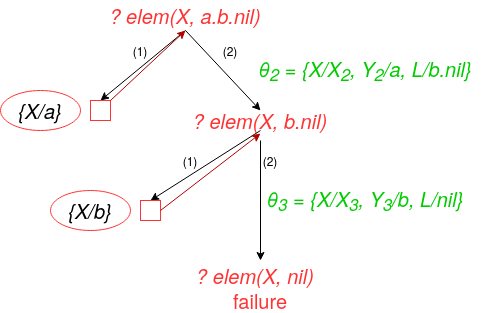
\includegraphics[height=200px]{./d1.png}
\end{center}
\begin{center}
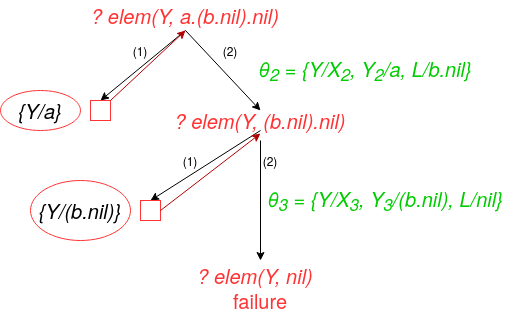
\includegraphics[height=200px]{./d2.png}
\end{center}
\begin{center}
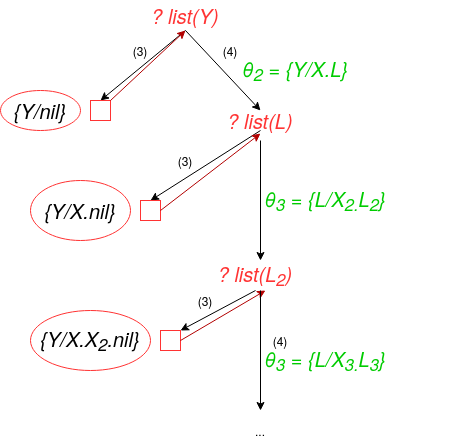
\includegraphics[height=300px]{./d3.png}
\end{center}
\begin{center}
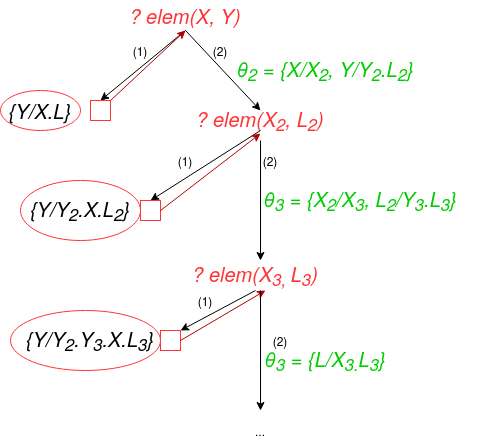
\includegraphics[height=300px]{./d4.png}
\end{center}
\end{document}
